\chapter{Appendix}

\section{Free Energy}
\label{sec:FE_app}
This article will try to give an intuitive review of the Free Energy as it is defined in statistical physics. We will see that Free Energy is a measure of a system's capacity to do work and that its minimization is a statistical necessity for a closed system. For the sake of clarity, I will use examples and interpretations which are not physically rigorous but help to develop a good understanding of the matter.

The toy example we are looking at is a two-state system which consists of ten "particles" which can take on two discrete energy values $E_0 = 0 J$ and $E_1 = 1 J$. A real-world analogon might be a collection electrons inside a magnetic field. Electrons whose spins are aligned parallel to the field correspond to particles in the lower energy level, while electrons with spins antiparallel to the field lines reside on the higher energy level (see Fig 1).

\begin{figure}
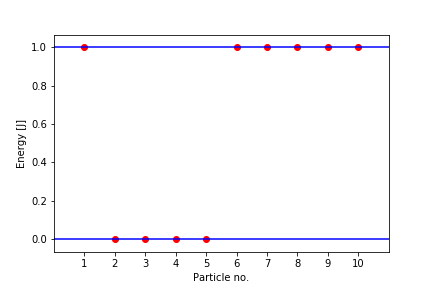
\includegraphics[scale=0.5]{images/FE_ex_1}
\caption{A two-level system with energy $E = 6J$}
\end{figure}

We will now consider one such system whose total energy is known to be $6J$. This means that six of its particles reside on the upper energy level while four particles occupy the lower level. One such possible system is shown in Figure 1. The committed reader may now pause for a second and consider for themselves if the displayed system appears to be in equilibrium or not. The (hopefully intuitive) answer is no. While we did not yet consider what "equilibrium" actually means, it may feel intuitive that in the given case, it means that the excited particles at energy $1J$ and the particles at energy $0J$ are somehow evenly distributed and do not clump together in one small region of the system.

In our case of of a 10-particle system with energy of $6J$, the number of possible microstates is 

$$\Omega_0(E = 6J) = {10\choose 6} = \frac{10!}{6!\cdot 4!} = 210.$$

In order to understand the main point of this article, we will apply a little trick whose use will become apparent later. We will split the system of ten particles into two compartments of five particles, the left of which we will call System A, while the other is System B (Fig. 2).

\begin{figure}
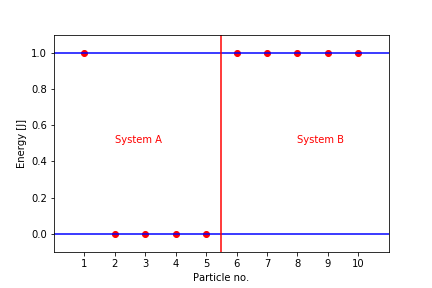
\includegraphics[scale=0.5]{images/FE_ex_2}
\caption{We separate the total System into two subsystems.}
\end{figure}

Next, we will go on to find the \textit{most likely} energy configurations of systems $A$ and $B$ such that their total energy $E = E_A + E_B$ equals $6 J$. We will find that the most probable energy configuration is the homogeneous state $E_A = E_B = 3J$ and that this state is reached by minimization of free energy or, equivalently, maximization of entropy.

\subsection{Finding the Probability for a given Energy of System A}

The question we are now trying to anser is:
\\
\\
For a system composed of two systems $A$ and $B$ as above, with total energy $E$, how likely is System $A$ to assume a specific energy level $E_A$?

In order to do this, we have to rely on one of the great postulates of statistical physics which we will accept as given (see Bibliography):
\\
\\
POSTULATE: In the equilibrium state, all possible microstates of a system are equally likely.
\\
\\
This postulate is also known as the \textit{The Fundamental Assumption of Statistical Mechanics}.
Using this postulate, our original question can be cast into mathematical form for the probability of System $A$ to have energy $E_A$. This is equal to the ratio of microstates that realize that energy to all other possible microstates that would result in a total energy of $E = 6J$:

$$W(E_A) \equiv (\text{Probability of System A assuming energy level }E_A) = \frac{\Omega_A(E_A)\cdot \Omega_B(E_B = E -E_A)}{\Omega_0(E)} \text{     (Eq. 1)}.$$

As this formula might feel intimidating for the mathematical layperson, I will go through it step by step:
$\Omega(E_A)$ is the number of microstates of System A that would realize a specific energy $E_A$. For our example (Figure 1), that energy corresponds to one particle in System A sitting on the upper energy level, thus $E_A = 1J$. For a total of 5 particles in System A, this is true for 5 different microstates, therefore $\Omega(E_A) = 5$. As we started with a known total energy $E = E_A + E_B$ (in our example 6J), requiring $E_A$ to be equal to $1J$ determines System B's energy $E_B = 5J$. The number of microstates that realize this is $\Omega(E_B = 5J) = 1$, as all particles in System B have to be in the upper state. The total number of different configurations such that $E_A$ is assumed by System A and $E_B$ by System B is therefore the product of the number of different microstates $\Omega_A(E_A)$ and $\Omega_B(E_B)$. The probability that any of these configurations is assumed is then equal to the ratio of that product with the number of all other possible microstates $\Omega_0(E)$ such that the total energy is $E$. In our case of 10 particles, six of which have to be in the upper energy level, that number is 210, as seen above. Therefore, the probability of finding our energy configuration in Figure 1 for a system at equilibrium is

$$W(E_A = 1J) = \frac{\Omega_A(E_A = 1 J)\cdot \Omega_B(E_B = 5J)}{\Omega_0(E = 6J)} = \frac{1\cdot 1}{210} \approx 0.005.$$

\subsection{Finding the most likely Energy for System A}

We are now interested in the most likely energy configuration for Systems $A$ and $B$ in the equilibrium state. The general idea is to find the value $\bar{E_A}$, for which $W(E_A)$ assumes a maximum value. This value can be found by setting the derivative of the probability function $W(E_A)$ to zero.

$$\frac{d}{d E_A} \ln (W(E_A)) = 0$$

The fact that we are deriving $\ln W(E_A)$ instead of $W(E_A)$ may not concern us here. The reason this is commonly done in statistical physics is that the maximum of the function $W(E_A)$ is at the same position as the maximum of the function $\ln W(E_A)$, while the latter is mathematically easier to deal with than the former. 

The energy $\bar{E_A}$ which maximizes $W(E_A)$ is then found to be the energy at which the energy is homogeneously dsitributed across the system:

$$\frac{\bar{E_A}}{f_A} = \frac{\bar{E_B}}{f_B} (Eq. 2),$$

where $f_i$ denotes the number of degrees of freedom of system i. In our example, the number of degrees of freedom is equal to the number of particles. What this means is that the most likely state a system at equilibrium will find itself in is a state of homogeneous energy distribution. This can be deduced from a purely statistical way of reasoning: The system at equilibrium can be found in each microstate with the same probability. The energy configuration the system will mos likely be found in is therefore the configuration which has the highest number of possible microstates. That energy configuration is however exactly the homogeneous case, where all imagined subsystem contain the same energy. More concretely, for our example:

$E_A = 1J \rightarrow \Omega_A(E_A)\cdot \Omega_B(E_B) = 5$

$E_A = 2J \rightarrow \Omega_A(E_A)\cdot \Omega_B(E_B) = 50$

$E_A = 3J \rightarrow \Omega_A(E_A)\cdot \Omega_B(E_B) = 100$

$E_A = 4J \rightarrow \Omega_A(E_A)\cdot \Omega_B(E_B) = 50$

$E_A = 5J \rightarrow \Omega_A(E_A)\cdot \Omega_B(E_B) = 5$


\begin{figure}
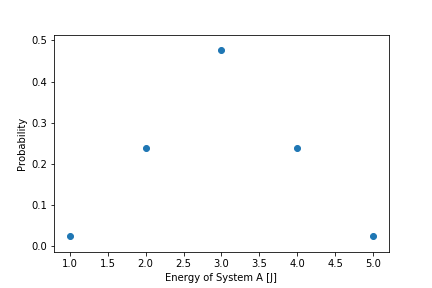
\includegraphics[scale=0.5]{images/FE_ex_3}
\caption{The probability for System A to have half of the total energy is highest.}
\end{figure}

The entropy is defined as 

$$S = k_B \ln \Omega(E).$$

Furthermore, entropy is an extensive property, i.e. the entropy of an ensemble of subsystems is the sum of the entropies of the single systems. 


Furthermore, entropy is an extensive property, i.e. the entropy of an ensemble of subsystems is the sum of the entropies of the individual systems:

$$\Omega(E) = \Omega_A(E_A)\cdot \Omega_A(E_A) \rightarrow S = k_B \ln \Omega(E) = k_B \ln \left( \Omega_A(E_A)\cdot \Omega_A(E_A) \right) \rightarrow S = S_A + S_B$$

Via the relations between the energy configurations of the subsystems and the number of microstates which would realize such configuration, it is easily seen that the entropy in this example is maximized by the homogeneous distribution of energies where $S_A = S_B$.

\subsection{Free Energy}

The (Helmholtz) Free Energy $F$ is defined as

$$F = E -TS,$$

where $E$ is the internal energy of the system and $T$ the (fixed) temperature of the system (equivalent to the system being in contact with a heat bath). As we have seen before, a closed system will always strive towards the equilibrium state which is equivalent to maximization of entropy. Given that $T$ is considered fixed, maximization of entropy thus corresponds to minimaztion of the free energy $F$. Note that the assumption of a given temperature $T$ is important here as otherwise $E$ and $T$ might be related via $$ \frac{1}{T} = \frac{dS}{dE}.$$


\subsection{Physical interpretation and work}

The above example was rather mathematical without much emphasis on physical interpretation. However, the concept of minimization of free energy $F$ does also have a very elegant physical interpretation.

As the minimum value of $F$ is reached when energy is homogeneously distributed across the system, a non-minimal value of $F$ is equivalent to local energy inhomogeneities. That is to say that the energy density varies from one point in the system to another. These changes in density can be described as energy gradients. Much like an electric potential is the necessary driver for flow of electric current, those energy gradients may create energy flows which, again, strive to reduce overall inhomogeneity. These energy flows can be harnessed to perform work. It is for this reason that free energy is generally considered as a measure of the energy with which a system can perform work. A system with high internal energy will not be able to perform work if that energy is completely homogeneously distributed.


\subsection{Temperature}

A homogeneous distribution of energy has as a direct consequence that the system at hand has the same temperature everywhere. This can easily be seen considering the equipartition theorem which relates the mean energy of a system in equilibrium with its temperature. For an ideal gas, the mean energy per atom is:

$$\bar{E} = \frac{3}{2}k_BT$$



\subsection{Conclusion}

Given the example considerations we can summarize the following:

1) The increase of entropy (and thus the decrease of free energy) is a statistical necessity. It describes a closed system's tendency to approach an equilibrium distribution with a homogeneous distribution of energy.

2) Free Energy is a measure of how far the system is from its equilibrium state. It is also a measure of the energy a system can harness to perform work.

2) This minimization of free energy $F$ can be interpreted on a physically level, as follows. Because a non-maximum value of the entropy (and thus non-minimal value of the Free Energy) corresponds to an inhomogeneous distribution of energy, minimization of $F$ is equivalent to saying that the system contains energy gradients with spatial extension larger than any single constituent (particle, say) of the system. These energy gradients are natural drivers of energy exchange, thus energy flow. This flow of energy can be harnessed to do work and thus drive motion. Internal energy alone does not give any information of a system's capacity to do work, while the distribution of energy within the system (i.e. its free energy) does.

4) By the above train of reasoning, the minimization of free energy corresponds to a well-known fact from biology: namely that every (living) system strives for homeostasis, i.e. internal equilibrium.


\subsection{Bibliography}

Torsten Fließbach: Statistische Physik IV


\subsection{Suggested Further Reading}

[1] E.T. Jaynes: Gibbs vs Boltzmann Entropies, American Journal of Physics \textbf{33}, 391 (1965).

Link: https://aapt.scitation.org/doi/pdf/10.1119/1.1971557?class=pdf

[2] E.T. Jaynes: The Gibbs Paradox. Link: https://bayes.wustl.edu/etj/articles/gibbs.paradox.pdf

\section{Energies and Logarithms}
\label{sec:EnergiesAndLogs}

Quite often we are dealing with logarithms of probability distributions and call them energies. In some cases, energies are minimized, in others they are maximized [Friston \& Kiebel: Predictive Coding under the Free Energy Principle].  I want to clarify where those ideas come from, and what they mean. \\

\noindent  In physics, energies and probability distributions are finely intertwined. Imagine the following problem (adapted from the Feynman lectures on Physics): Given the density of the atmosphere at ground level, how dense are the air molecules at a given altitude $h$? The only reason why the density of the air is higher at ground level than at higher altitudes is due to the earth's gravitational force, such that at ground level you have to withstand the pressure created by all the air molecules above you. Those molecules are pulled down by the earth's gravitational field. Analogously, you might as well just talk about an air molecule's potential energy: The higher up, the more potential energy. It turns out that the air density $n$ density at any height $h$ is exactly a function of the potential energy at that height:

\begin{align*}
n = \alpha e^{-\beta E_{pot}},
\end{align*}
with some constants $\alpha, \beta$. \\

\noindent Now consider this question: Given a box full of air with temperature $T$, what is the probability for particle to have velocity $v$? The answer is

\begin{align*}
f(u)du = const \cdot e^{-\beta E_{kin}(u)}du
\end{align*}
for a velocity between $u$ and $u+du$. Thus, the \textit{probability distribution} (or more accurately \textit{probability density function}) of the velocities is

\begin{align*}
f(u) = const \cdot e^{-\beta E_{kin}(u)}.
\end{align*}

It turns out that basically any probability density function which describes the distribution of a quantity of interest in a thermodynamic setting with conservative forces can be written in terms of the corresponding kinetic and potential energies, as above. [Feynman, Statistical Physics] \\

\noindent Given a probability distribution of the form $p(x) = e^{-E(x)}$ (omitting constants), one can easily see that $E(x) = -\ln p(x)$. As in Bayesian Inference, we are dealing a lot with the logarithms of probability distributions, it has become convenient to refer to them as energies. It is however important to note that those \textit{energies} do not usually have a physical interpretation, or any other meaningful interpretation. The expression comes purely from the analogy with statistical physics.

\section{Identities}
\begin{align}
FE &= D_{KL}(q(z)||p(z|y)) - \ln p(y) \\
&= -ELBO \\
& = - \left<\ln p(y,z) -\ln q(z) \right>_{q(z)}.
\end{align}

\section{Ergodicity}
Probabilities do not exist. They only exist in repetition experiments. Blablabla